\documentclass{report}
\usepackage[spanish]{babel}
\usepackage[utf8]{inputenc}
\usepackage{graphicx, longtable}

\begin{document}
    \begin{titlepage}
        \centering
        
\includegraphics[width=0.6\textwidth]{./img/miscelanio/logo.jpg}\\
        \vspace{1cm}
        \LARGE Sistemas de Gestión de Seguridad de Sistemas de Información\\
        \vspace{0.5cm}
        \Large Ingeniería Informática de Gestión y Sistemas de Información\\
        \vspace{3cm}
        \Huge Sistema Web\\
        \vspace{2.5cm}
        \Large Autores:\\
        \vspace{0.2cm}
        \large Xabier Gabiña\\
        \large Ainhize Martinez\\
        \large Marcos Martín\\
        \vfill
        \today
    \end{titlepage}
    \tableofcontents
    \chapter{Introduccion}
        El objetivo de este trabajo no es otro que el de desarrolar un  sistema web usando las tecnologias \textbf{HTML, CSS, JavaScript, PHP, MySQL(MariaDB) y Docker} con el que se pretende alcanzar el desarrolar una pagina web que permita \textbf{registrarse, iniciar sesion, modificar datos del usuario, añadir elementos, generar un listado de elementos y modificar dichos elementos} en primera instancia todo de forma insegura para posteriormente poner en practica lo aprendido a lo largo de la asignatura sobre seguridad.
        \\\\
        Todo esto sera puesto en practica mediante el desarroyo de un videoclub en linea que incluye todas estas funcionalidad el cual nos servira para mostrar los conocimientos en la materia a trabajar.
    \chapter{Manual de Usuario}
        \section{Registro}
            \begin{figure}[h!]
                \centering
                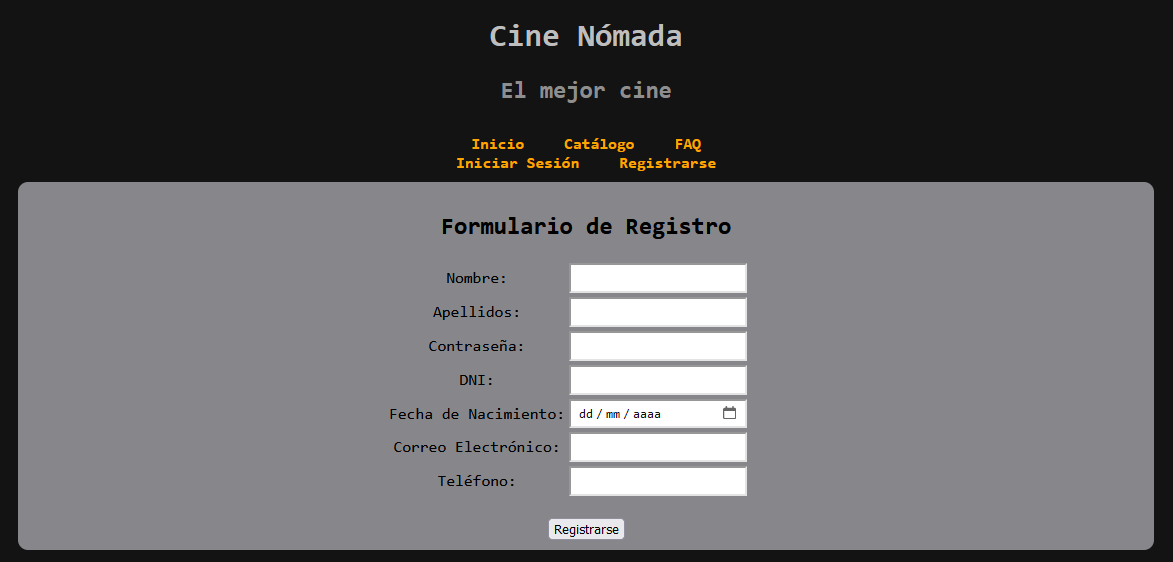
\includegraphics[width=\textwidth]{./img/ui/register.png}
                \caption{Formulario de Registro}
            \end{figure}
            Como podemos ver en la Figura 3.1 el formulario de registro consta de siete campos \textbf{Nombre, Apellidos, Contraseña, DNI, Fecha de Nacimiento, Correo Electronico y Telefono.} A excepcion de los apellidos todos ellos son necesarios para tramitar el registro mediante el boton al final del formulario. Una vez se haya pulsado dicho boton el formulario sera verifiado mediante una funcion JavaScript que verificara la correccion de los datos y permitira el envio de los mismos al servidor para su posterior registro en la base de datos.
        
        \clearpage
        \section{Inicio de Sesion}
            \begin{figure}[h!]
                \centering
                
\includegraphics[width=\textwidth]{./img/ui/login.png}
                \caption{Formulario de Inicio de Sesion}
            \end{figure}
            Como se aprecia en la Figura 3.2 el formulario de inicio de sesion, en este caso, consta de dos campos \textbf{Correo Electronico y Contraseña.} Estos campos sirven para verificar la identidad del usuario ya que no puede haber dos correos identicos en el sistema y la contraseña solo debe de conocerse por el dueño de la cuenta.
            \\\\
            Una vez introducidos los datos y presioado el boton, si los datos son correctos, se validara la sesion, se recargara la pagina y se nos mostraran nuevas opciones en la barra de navegacion.

        \clearpage
        \section{Editar datos personales}
            \begin{figure}[h!]
                \centering
                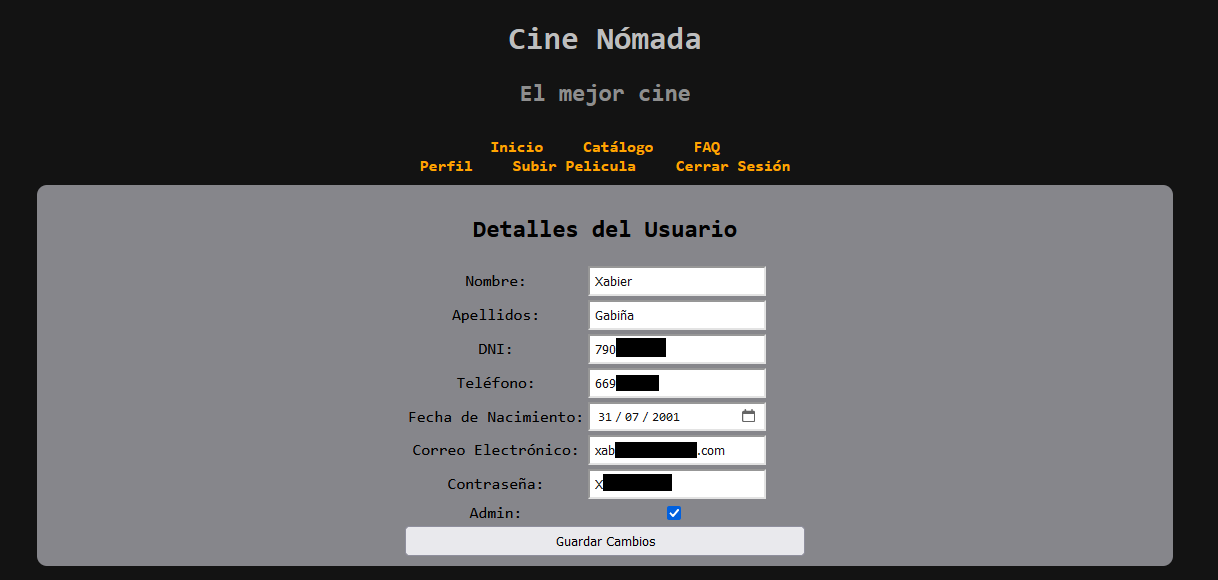
\includegraphics[width=\textwidth]{./img/ui/perfil.png}
                \caption{Formulario de actualizacion de datos personales}
            \end{figure}
            El formulario de la Figura 3.3 solo es accesible una vez identificado, el usuario, en el sistema. Este formulario mostrara la informacion actual del usuario, con sesion activa, en la base de datos y permitira su actualizacion mediante los campos del formulario para su posterior actualizacion mediante el boton al final del mismo.

            \clearpage
        \section{Catalogo}
            \begin{figure}[h!]
                \centering
                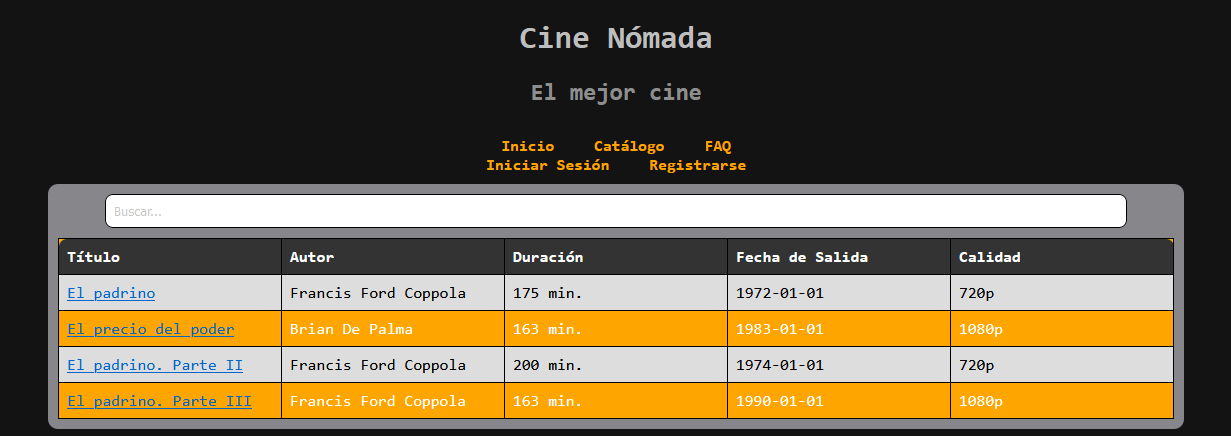
\includegraphics[width=\textwidth]{./img/ui/catalogo.png}
                \caption{Tabla de peliculas}
            \end{figure}  
            La tabla que podemos ver en la Figura 3.4 es en la que se listan las peliculas registradas en el sistema. Esta tabla consta de cinco columnas: \textbf{Titulo, Autor, Duracion, Fecha de Salida y Calidad.} 
            \\\\
            Si nos fijamos en la columna Titulo podemos ver que es un hiperenlace el cual esta ligada a la funcionalidad de editar pelicula que se desarrola en la siguiente subseccion.

            \clearpage
            \subsection{Editar pelicula}
                \begin{figure}[h!]
                    \centering
                    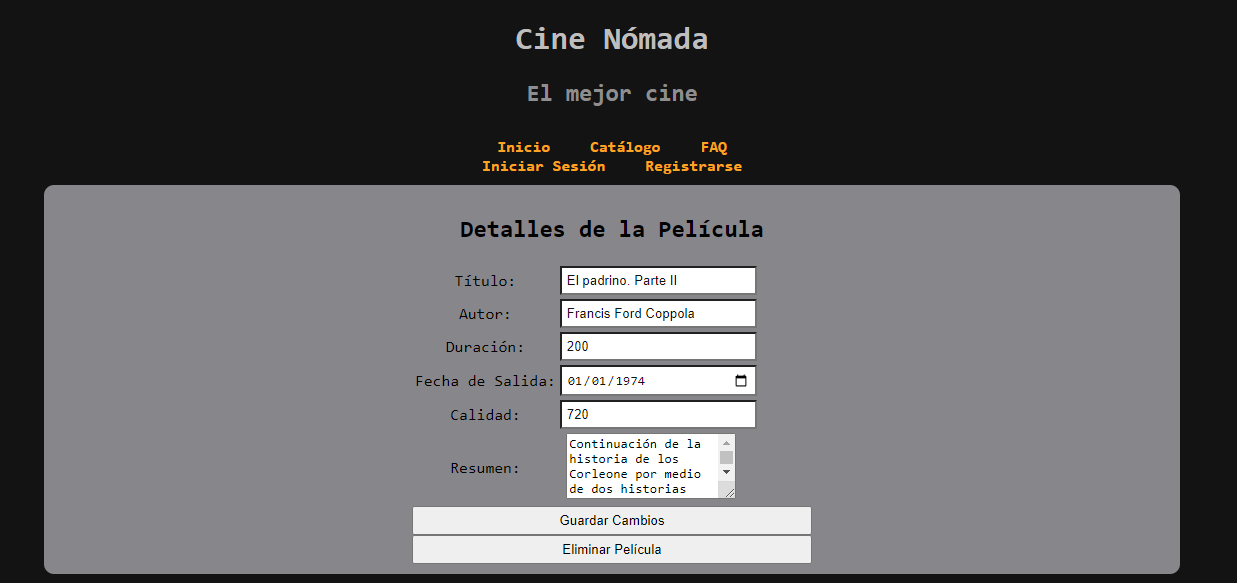
\includegraphics[width=\textwidth]{./img/ui/editarp.png}
                    \caption{Formulario de registro de pelicula}
                \end{figure}
                Mediante el formulario Figura 2.5 se nos muestra los datos que contienen las peliculas del sistema y se nos da las opciones tanto de editarlos como de eliminarlos del sistema.

        \clearpage
        \section{Subir pelicula} 
            \begin{figure}[h!]
                \centering
                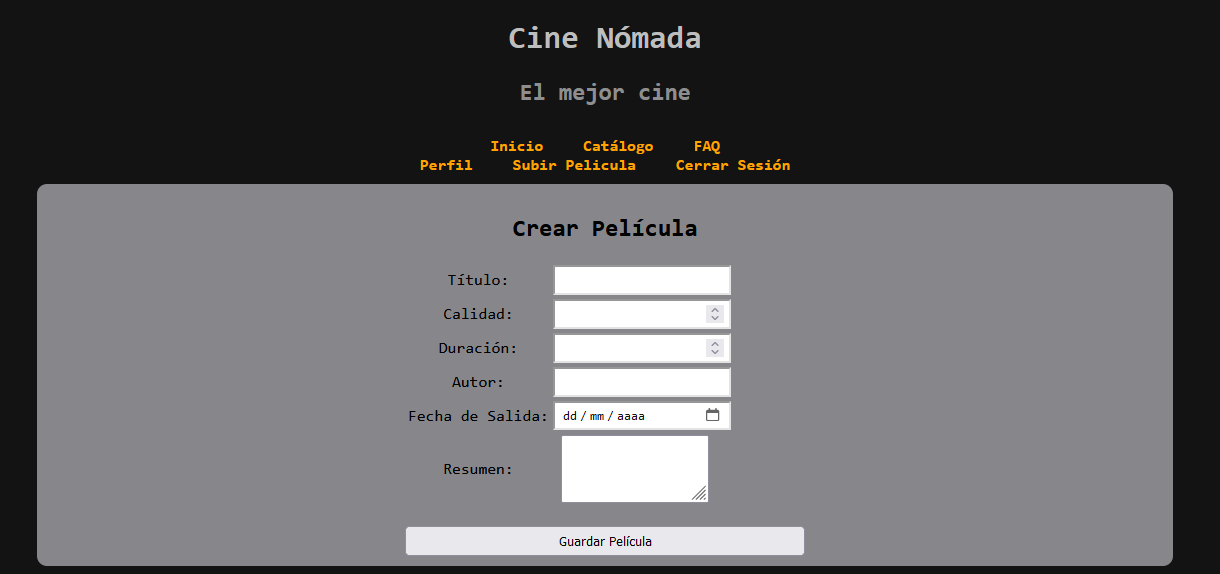
\includegraphics[width=\textwidth]{./img/ui/subirp.png}
                \caption{Formulario de registro de pelicula}
            \end{figure}
            Mediante este formulario visible en la Figura 2.6 se le permite a todo usuario subir una nueva pelicula al sistema y que esta sea mostrada junto al resto en el Catalogo lo cual a su vez tambien permite la modificacion de la misma.
\end{document}